% Document settings
\documentclass[a4paper,11pt]{article}

% Packages
  % math formulas
\usepackage{amsmath,amsthm,amssymb}
  % graphics
\usepackage{graphicx}
\usepackage{wrapfig}
  % plots
\usepackage{pgfplots}
  % other
\usepackage[warn]{mathtext}
\usepackage{cmap}
\usepackage[T1,T2A]{fontenc}
\usepackage[utf8]{inputenc}
\usepackage[english,russian]{babel}
\usepackage{icomma}

% Package settings
%% graphicx
\graphicspath{{Pictures/}}
\DeclareGraphicsExtensions{.pdf,.png,.jpg}
%% pgfplots
\pgfplotsset{width=10cm,compat=1.9}

% Title
\title{Отчет о выполнении работы №2.3.1\\Получение и измерение вакуума}
\author{Воейко Андрей Александрович, Б01-109}
\date{Долгопрудный, 2022}

% Document
\begin{document}
\maketitle
\newpage
\section{Аннотация.}
В работе измеряется объем форвакуумной и высоковакуумной частей установки, а также определяется скорость откачки системы в стационарном режиме.
\section{Теоретические сведения и экспериментальная установка.}
По степени разрежения вакуумные установки принято делить на три класса:
\begin{itemize}
        \item Низковакуумные~--- до $10^{-2}$--$10^{-3}$ торр.
        \item Высоковакуумные~--- до $10^{-2}$--$10^{-3}$ торр.
        \item Сверхвысокого вакуума~--- до $10^{-2}$--$10^{-3}$ торр.
\end{itemize}
В данной работе исследуются традиционные методы откачки механическим форвакуумным насосом до давления $10^{-2}$ торр и диффузионным масляным насосом до давления $10^{-5}$ торр, а также методы измерения вакуума в этом диапазоне.
\subsection{Экспериментальная установка.}
Установка изготовлена из стекла и состоит из фовакуумного баллона (ФБ), высоковакуумного диффузионного насоса (ВН), высоковакуумного баллона (ВБ), масляного (М) и ионизационного (И) манометров, термопарных манометров (М$_{1}$ и М$_{2}$), форвакуумного насоса (ФН) и соединительных кранов К$_{1}$, К$_{2}$ ... К$_{6}$ (рис.~\ref{fig:img1}). Кроме того, в состав установки входят: вариатор (автотрансформатор с регулируемым выходным напряжением), или реостат и амперметр для регулирования тока нагревателя диффузионного насоса.
\subsubsection{Краны.}
Все краны вакуумной установки~--- стеклянные. Стенки кранов тонки, пробки кранов полые и составляют одно целое с рукоятками. Кран К$_{1}$ используется для заполнения форвакуумного насоса и вакуумной установки атмосферным воздухом. Во время работы установки он должен быть закрыт. Трехходовой кран К$_{2}$ служит для соединения форвакууминого насоса с установкой атмосферой. Кран К$_{3}$ отделяет высоковакуумную часть установки от форвакуумной. Кран К$_{4}$ соединяет между соьой колена масляного манометра. Он должен быть открыт во все время работы установки и\\
\begin{center}
\begin{wrapfigure}{r}{1\textwidth}
  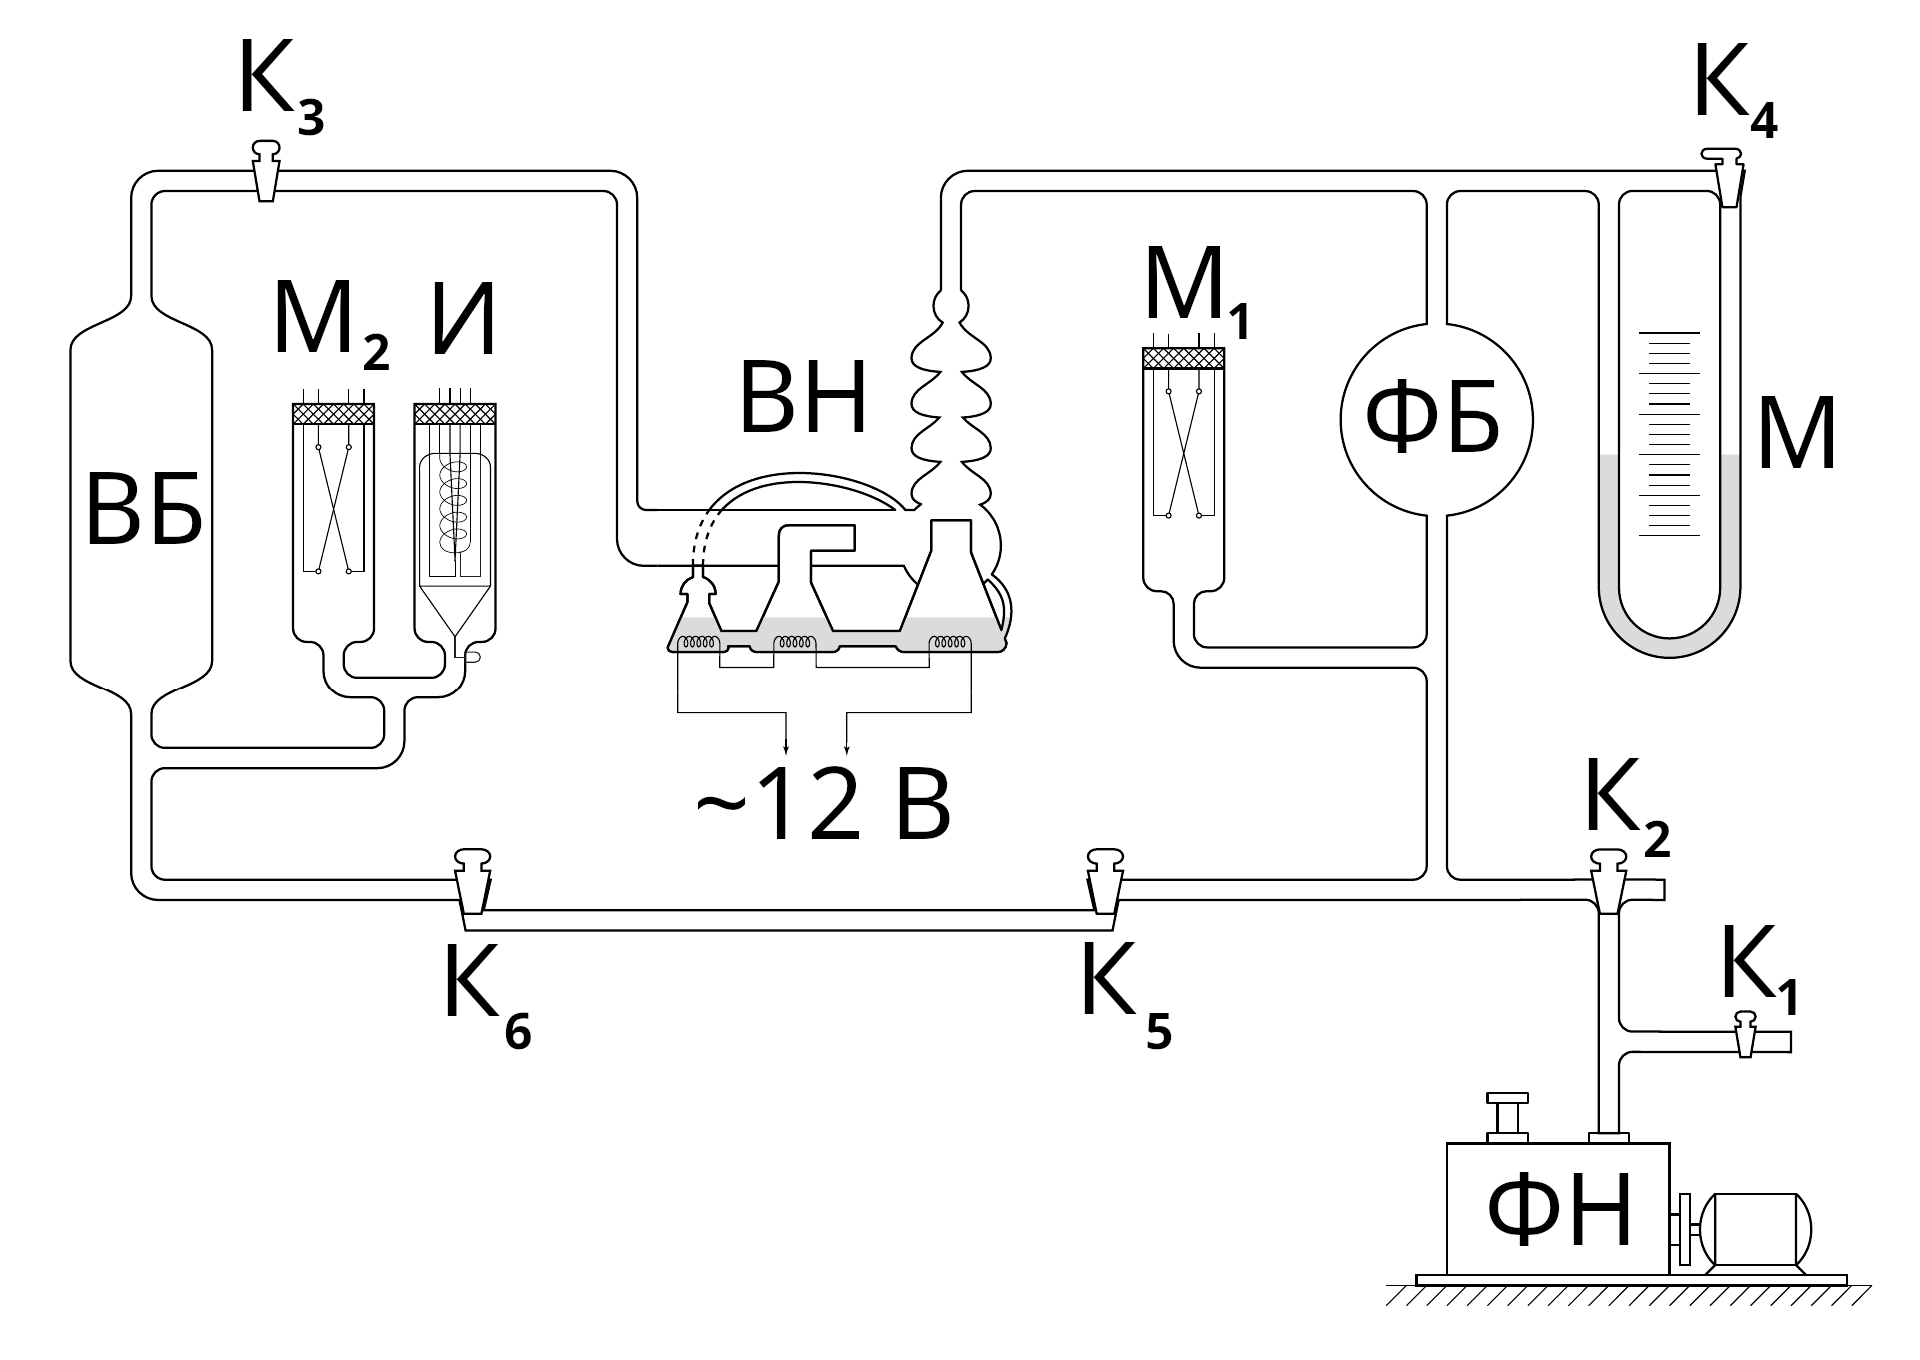
\includegraphics[scale = 0.31]{scheme1.png}
  \caption{Схема экспериментальной установки.}
  \label{fig:img1}
\end{wrapfigure}
\end{center}
закрывается лишь во время работы установки и закрывается лишь при измерении давления в форвакуумной части. Краны К$_{5}$ и К$_{6}$ стоят по концам капиояра и соединяют его с форвакуумной и высоковакуумной частями установки. Суммарный объем обоих кранов и капиляра $50\ см^{3}$. Диаметр капиляра $0,8\ мм$. Его длина $108\ мм$.
\subsubsection{Форвакуумный насос.}
Устройство и принцип действия ротационного форвакуумного насоса, ипользующегося в данной работе, изображены на рис.~\ref{fig:img2}.\\
\begin{center}
\begin{wrapfigure}{r!}{1\textwidth}
  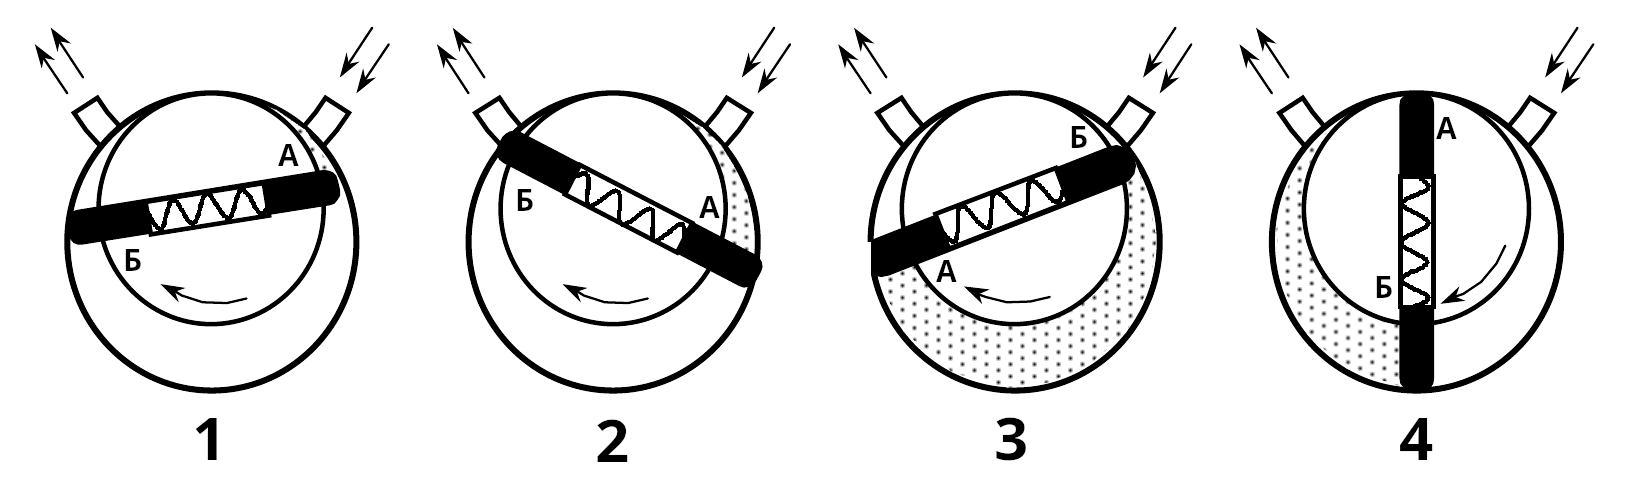
\includegraphics[scale = 0.35]{scheme2.png}
  \caption{Схема действия ротационного пластинчатого форвакууминого насоса.}
  \label{fig:img2}
\end{wrapfigure}
\end{center}
Насос состоит из ротора, расположенного эксцентрично в цилиндре. В роторе есть прорезь, в которой располагаются способные предвигаться в нем пластины. В ходе вращения в цилиндре образуются две полости~--- увлекаемые пластинами <<А>> и <<Б>> соответственно. На первом и втором рисунках пластина <<А>> втягивает воздух из входной трубки в полость. На третьем полость отделяется от трубки пластиной <<Б>>, а на четвертом пластина <<Б>> заталкивает воздух в выходную трубку.
\subsubsection{Диффузионный насос.}
Откасчивающее действие диффузионного насоса основано на диффузии молекул разреженного воздуха в струю паров масла. Попавшие в струю модекулы газа увлекаются ею и уже не возвращаются назад. Устройство этого насоса изображено на рис.~\ref{fig:img3}.\\
\begin{center}
\begin{wrapfigure}{r!}{1\textwidth}
  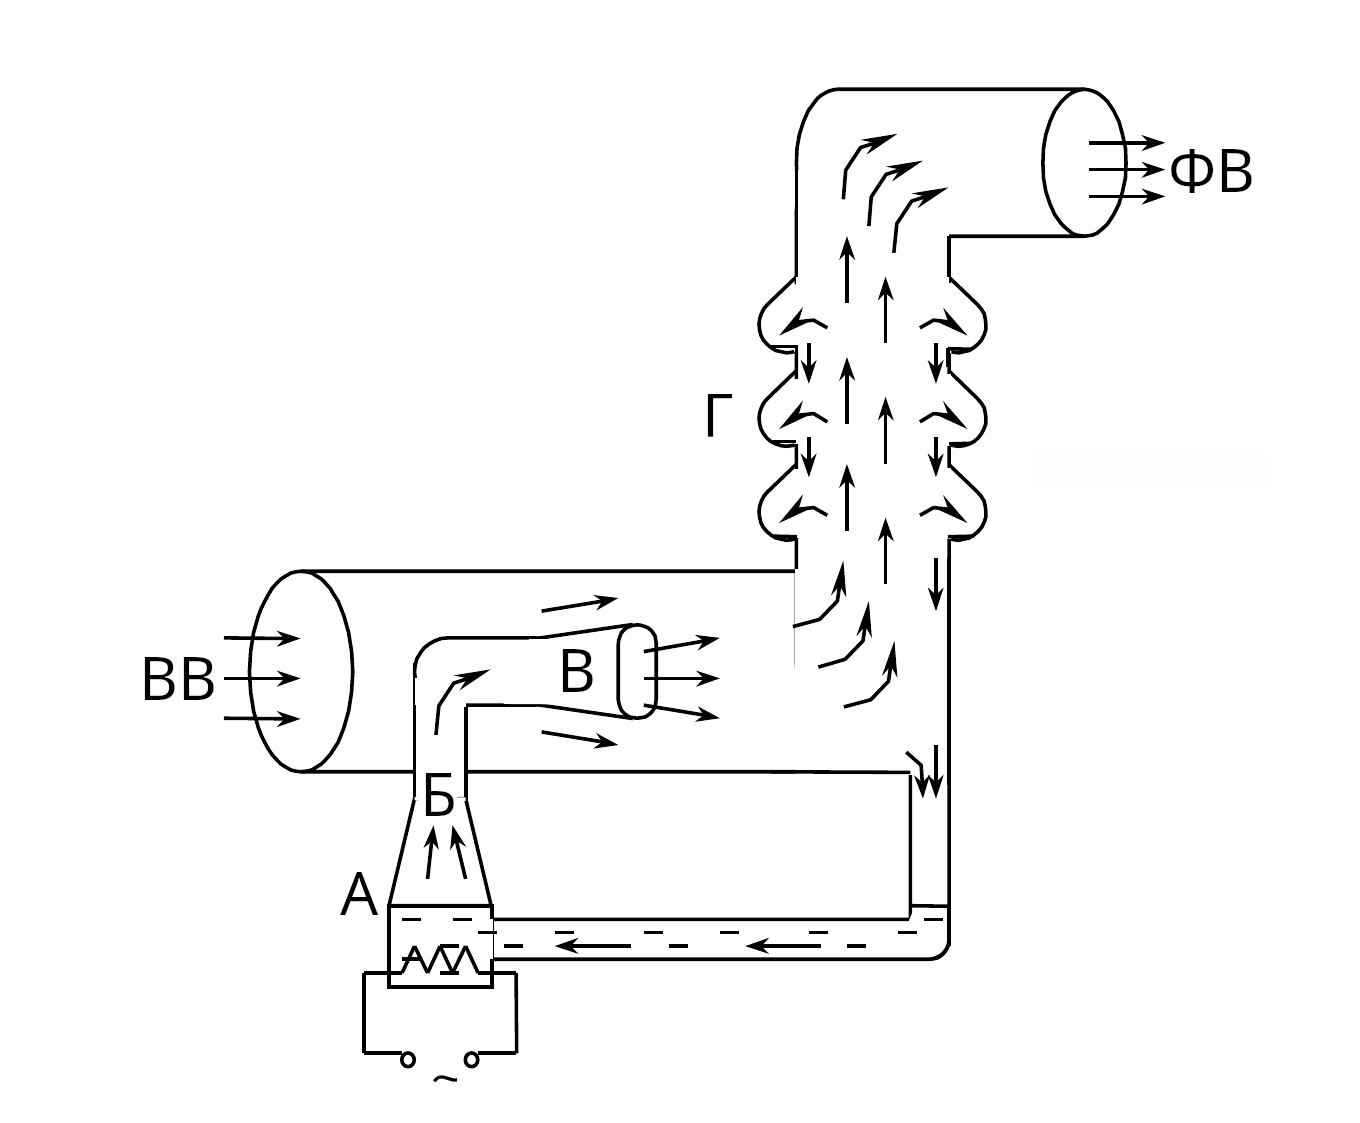
\includegraphics[scale = 0.4]{scheme3.png}
  \caption{Схема действия ротационного пластинчатого форвакууминого насоса.}
  \label{fig:img3}
\end{wrapfigure}
\end{center}
Масло нагревается электрической печкой. Пары масла поднимаются по трубе Б и вырываются из сопла В. Струя паров увлекает молекулы газа, которые поступают из откачиваемого сосуда через трубу ВВ. Дальше смесь попадает в вертикальную трубу Г. Здесь масло осаждается на стенках трубы и маслосборников и стекает вниз, а оставшийся газ через трубу ФВ откачивается форвакуумным насосом. Диффузионный насос работает наиболее эффективно при давлении, когда длина свободного пробега молекул воздуха примерно равна ширине кольцевого зазора между соплом В и стенками трубы ВВ. В этом случае пары масла увлекают молекулы воздуха из всего сечения зазора.
\subsubsection{Процесс откачки.}
Производительность насоса определяется скоростью откачки $W\ (л/с)$: $W$~--- это объем газа, удаляемого из сосуда при данном давлении за единицу времени. Скорость откачки фовакуумного насоса равна емкости воздухозаборной камеры, умноженной на число оборотов в секунду.\\
Рассмотрим обычную схему откачки. Разделим вакуумную систему на две части: <<откачиваемый объем>> (в состав которого включим используемые для работы части установки) и <<насос>> к которому кроме самого наоса, отнесем трубопроводы и краны, через которые производится отчкачка нашего объема. Обозначим через $Q_{д}$ количество газа, десорбирующегося с поверхности откачиваемого объема в единицу времени, через $Q_{и}$~--- количество газа, проникающего в этот объем извне~--- через течи.
\section{Результаты измерений и обработка данных.}
\section{Выводы.}
\end{document}
